\Chapter{Rácsok részei}

A rácsoknak három különböző része van: a lapok, az élek és a csúcsok. Minden lap két dimenziós felület élek által határolva. Minden él egy dimenziós szakasz aminek mind a két végén csúcsok találhatóak. Minden csúcs nulla dimenziós pont. 

\begin{figure}[h]
\centering
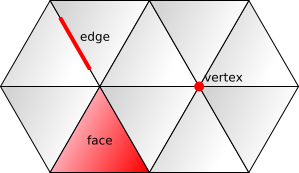
\includegraphics[scale=0.5]{kepek/img31.png}
\caption{A rácsok részei}
\label{fig:img31}
\end{figure}

\noindent A játékok nagy többségében közös az, hogy a rácsoknak csak az egyik részére koncentrálnak. A nyugati játékoknál mint a sakk vagy a dáma a rácsnak a lap részén van a fókusz ellentétben a keleti játékokkal mint a Go vagy a Csillaghalma (Chinese Checkers), ahol a csúcsokon van.
\newline
\newline Lapok, élek és csúcsok feltűnnek a különböző poligonokból álló  térképek esetén is. Egy olyan algoritmus ami a lapok, élek vagy csúcsok alapján működik de nincs szükség koordinátákra az működni fog ilyen térképek esetén is.

\begin{figure}[h]
\centering
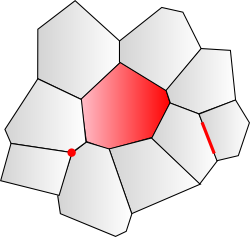
\includegraphics[scale=0.5]{kepek/img32.png}
\caption{Különböző poligonokból álló térkép.}
\label{fig:img32}
\end{figure}

\noindent A rácsok és a poligonális térképek átalakíthatóak gráf struktúrákra azáltal, hogy minden lapból csomópontot és minden lapok közötti élből pedig a csomópontok közötti gráf éleket készítünk. A gráf struktúra megengedi számunkra, hogy gráf algoritmusokat (például: legrövidebb út) használjunk a térképen.

\section*{Használatuk játékokban}

A számítógépes játékok mind a három típust használhatják, de a lap a leggyakoribb. Épületek, terület típusok (fű, sivatag, stb.) és a terület birtoklás a lapokat használja. Terület határok és az “áramlás” (“flow”) algoritmusok (ami szimulálja az áramlását a víznek, embereknek, termékeknek, stb. a szomszédos csempék között) használják az éleket. Az utakhoz lehet használni a lapokat és az éleket is.